\section{Commit Types}
\label{sec:type}

\subsection{Previous Works}
Previous works primarily characterize commits based on metadata.
Alali et al.\cite{Alali} define commit properties by size -- lines of code, number of code blocks, and file count -- as well as extracted terms from commit messages.
%\review{It would have been interesting to validate the results in [1] based on the taxonomy refinement and analyze/compare the differences. This can improve the significance of the work.}
Kaur et al. \cite{Kaur2018} propose a classifier for labeling commit type -- bug repair, feature addition, and general -- based on commit messages.
However, commit message alone is not enough to effectively categorize commits. While a commit message can indicate developer intent, it will not necessarily address all the major code changes. 
Dragan et al. \cite{Dragan} perform categorization over commit code, stereotyping added and removed methods to form a descriptor for commit change.
Solely focusing on code to determine commit characteristics can often introduce additional noise. While commit messages are brief summaries indicating the central goal of the commit, code diffs capture details that do not affect high-level categorization. Further, determining commit type, based entirely on code, becomes difficult on extremely large commits, where a commit message may provide all of the information needed.

Hindle et al. \cite{Hindle_cate} propose a taxonomy based on the maintenance tasks to categorize large commits.
This categorization uses maintenance attributes first introduced by Swanson et al. \cite{Swanson}.
They further map the categories to the taxonomy of Mauczka et al.\cite{Mauczka}, dividing changes into high-level classes of software maintenance: \textit{adaptive}, \textit{perfective}, and \textit{corrective}. The taxonomy is then used for automatic categorization \cite{Hindle_auto}. Based on the results and methodology, our work proposes a refinement of the taxonomy presented by Hindle et al, adapted to reduce ambiguity between categories, and to support tagging small commits.


\subsection{A Refined Categorization}
\begin{table}[htbp]
  \centering
  \caption{Refined Categorization}
    \begin{tabular}{|p{6em}|p{9em}r|}
    \hline
    Type  & \multicolumn{1}{p{9em}|}{Hindle's Definition} & \multicolumn{1}{p{12.5em}|}{Our Explanation} \\
    \hline
    Branch & \multicolumn{2}{p{21.5em}|}{If the change is primarily to do with branching or working off the main development trunk of the version control system.} \\
    \hline
    Bug fix & \multicolumn{1}{p{9em}|}{One or more bug fixes.} & \multicolumn{1}{p{12.5em}|}{A change that is reported in the developing log, change log or with expressions in commit message that indicates it is a correction of unexpected behavior.} \\
    \hline
    Build & \multicolumn{2}{p{21.5em}|}{If the focus of the change is on the build or configuration system files. (such as Makefiles).} \\
    \hline
    Clean up & \multicolumn{2}{p{21.5em}|}{Cleaning up the source code or related files. This includes activities such as removing non-used functions.} \\
    \hline
    Legal & \multicolumn{2}{p{21.5em}|}{A change of license, copyright or authorship.} \\
    \hline
    Cross & \multicolumn{2}{p{21.5em}|}{A cross cutting concern is addressed (like logging).} \\
    \hline
    Data  & \multicolumn{2}{p{21.5em}|}{A change to data files required by the software (different from a change to documentation).} \\
    \hline
    Debug & \multicolumn{2}{p{21.5em}|}{A commit that adds debugging code.} \\
    \hline
    Documentation & \multicolumn{2}{p{21.5em}|}{A change to the system's documentation.} \\
    \hline
    External & \multicolumn{2}{p{21.5em}|}{Code that was submitted to the project by developers who are not part of the core team of the project.} \\
    \hline
    Feature Add & \multicolumn{1}{p{9em}|}{An addition/implementation of a new feature.} & \multicolumn{1}{p{12.5em}|}{New function/methods/class implemented, impacting functionality.} \\
    \hline
    Indentation & \multicolumn{2}{p{21.5em}|}{Re-indenting or reformatting of the source code.} \\
    \hline
    Initialization & \multicolumn{2}{p{21.5em}|}{A module being initialized or imported (usually one of the first commits to the project).} \\
    \hline
    Internationa- lization & \multicolumn{2}{p{21.5em}|}{A change related to its support for languages other-than-English.} \\
    \hline
    Source Control & \multicolumn{2}{p{21.5em}|}{A change that is the result of the way the source controls system works, or the features provided to its users (for example, tagging a snapshot).} \\
    \hline
    Maintenance & \multicolumn{1}{p{9em}|}{A commit that performs activities common during maintenance cycle (different from bug fixes, yet, not quite as radical as new features).} & \multicolumn{1}{p{12.5em}|}{Functional changes without feature add and do not have evidence to be considered a bug fix, including performance Improvement and feature extension.} \\
    \hline
    Merge & \multicolumn{2}{p{21.5em}|}{Code merged from a branch into the main trunk of the version control system; it might also be the result of different and non-necessarily related changes committed simultaneously to the version control system.} \\
    \hline
    Module Add & \multicolumn{2}{p{21.5em}|}{If a module (directory) or files have been added to a project.} \\
    \hline
    Module Move & \multicolumn{2}{p{21.5em}|}{When a module or files are moved or renamed.} \\
    \hline
    Module Remove & \multicolumn{2}{p{21.5em}|}{Deletion of module or files.} \\
    \hline
    {Platform Specific} & \multicolumn{2}{p{21.5em}|}{A change needed for a specific platform (such as different hardware or operating system).} \\
    \hline
    Refactoring & \multicolumn{1}{p{9em}|}{Refactoring of portions of the source code.} & \multicolumn{1}{p{12.5em}|}{Relocation of part of code. Restructuring.
    Extract a part of code out of a function and create a new function.} \\
    \hline
    Rename & \multicolumn{2}{p{21.5em}|}{One or more files are renamed, but remain in the same module (directory).} \\
    \hline
    Testing & \multicolumn{2}{p{21.5em}|}{A change related to the files required for testing or benchmarking.} \\
    \hline
    Token Replace & \multicolumn{2}{p{21.5em}|}{An token (such as an identifier) is renamed across many files (e.g. change the name or a function).} \\
    \hline
    Versioning & \multicolumn{2}{p{21.5em}|}{A change in version labels of the software (such as replacing ``2.0'' with ``2.1'').} \\
    \hline
    \end{tabular}%
  \label{tab:categorization}%
\end{table}%



To analyze the difference in purpose between breakers and neutrals, we need an accurate categorization for commits.
Although we leverage Hindle's categorization, it was originally designed for usage only on large commits.
Several change types such as Maintenance, Bug Fix, Debug and Refactoring were too broadly defined when applied to smaller commits, and at times needed to be accompanied by other categories to fully classify the commit change.

Our analysis leads to a refinement of Hindle's categories, and the identification of the commits that warrant defining new categories for comprehensive classification.
These modifications result in variations in category frequency from those found by Hindle et al. \cite{Hindle_cate}. This indicates, in part, significant changes in category definitions. For example, out of the 2000 commits that they analyzed, 2\% were tagged as maintenance while in our analysis it's more than 40\%.
This result is surprising, as other studies  \cite{dodaro2015government,redman2008weapon,koskinen2009software} report that 75\% of software development budgets are dedicated to maintenance. Another contributing factor for the variation in category frequency is our inclusion of small commits. Along with the new taxonomy, we provide results that describe the relationship between commit size and purpose.

Table \ref{tab:categorization} shows the refined taxonomy.
Specifications for types are as follows:

\textbf{Bug Fix:} In small commits, the lack of descriptive code makes it hard to differentiate between Bug Fix and Maintenance categorization. 
As a result, we have to rely on commit messages and project change logs. 
For example, if a commit message mentions fixing an existing issue, it should be tagged a Bug Fix. We also thoroughly examine previous software revisions, to see if the commit is added in response to flaws in recent code.
While we take these steps to better identify Bug Fixes, some commits are still too vague to be clearly tagged Maintenance or Bug Fix. 
Further improvement and definition of rules are needed to make the tagging more definitive on small commits.

\textbf{Feature Add:} We found that Hindle's definition of a Feature Add is under-specified for smaller commits.
This may be because new features are easily identifiable in larger commits via the commit message, whereas in small code changes, new features can be a single non-utility function or method. We include this in our refined definition of Feature Add.

\textbf{Maintenance:} This is the most under-specified type in the original taxonomy.
Cross validation indicates more than half of the commits with inconsistent tags are with Maintenance. 
Thus, we consult with Hindle et al. regarding this tag.
According to our discussion, this should be better translated to ``minor perfective changes'' which is different from the maintenance tasks we generally use.
Since the original definition can cause confusion due to little specification, we define it as function \& efficiency improvements, additions of utility functions, or minor modifications without new methods or error corrections.
For example, memory cleaning is tagged as Maintenance because it is a performance improvement. 


\textbf{Refactoring:} 
We specify Refactoring as relocation, restructuring of code without altering how the code functions, such as extracting code to form a new function, relocating code hunks within or across files, or other changes to reduce code redundancies.
They do not change functionality or efficiency.

Note that by our definition, breakers and neutrals can not be merge or orphan commits, as we study the impact of a commit by comparing two revisions: the one it changes and the one it produces.
As a result, there are no commits in the Branch and Initialization categories.
\subsection{The Difference Between Categories with Respect to Software Quality}


\subsection{Independent Change}

\begin{figure}[htbp]
\centerline{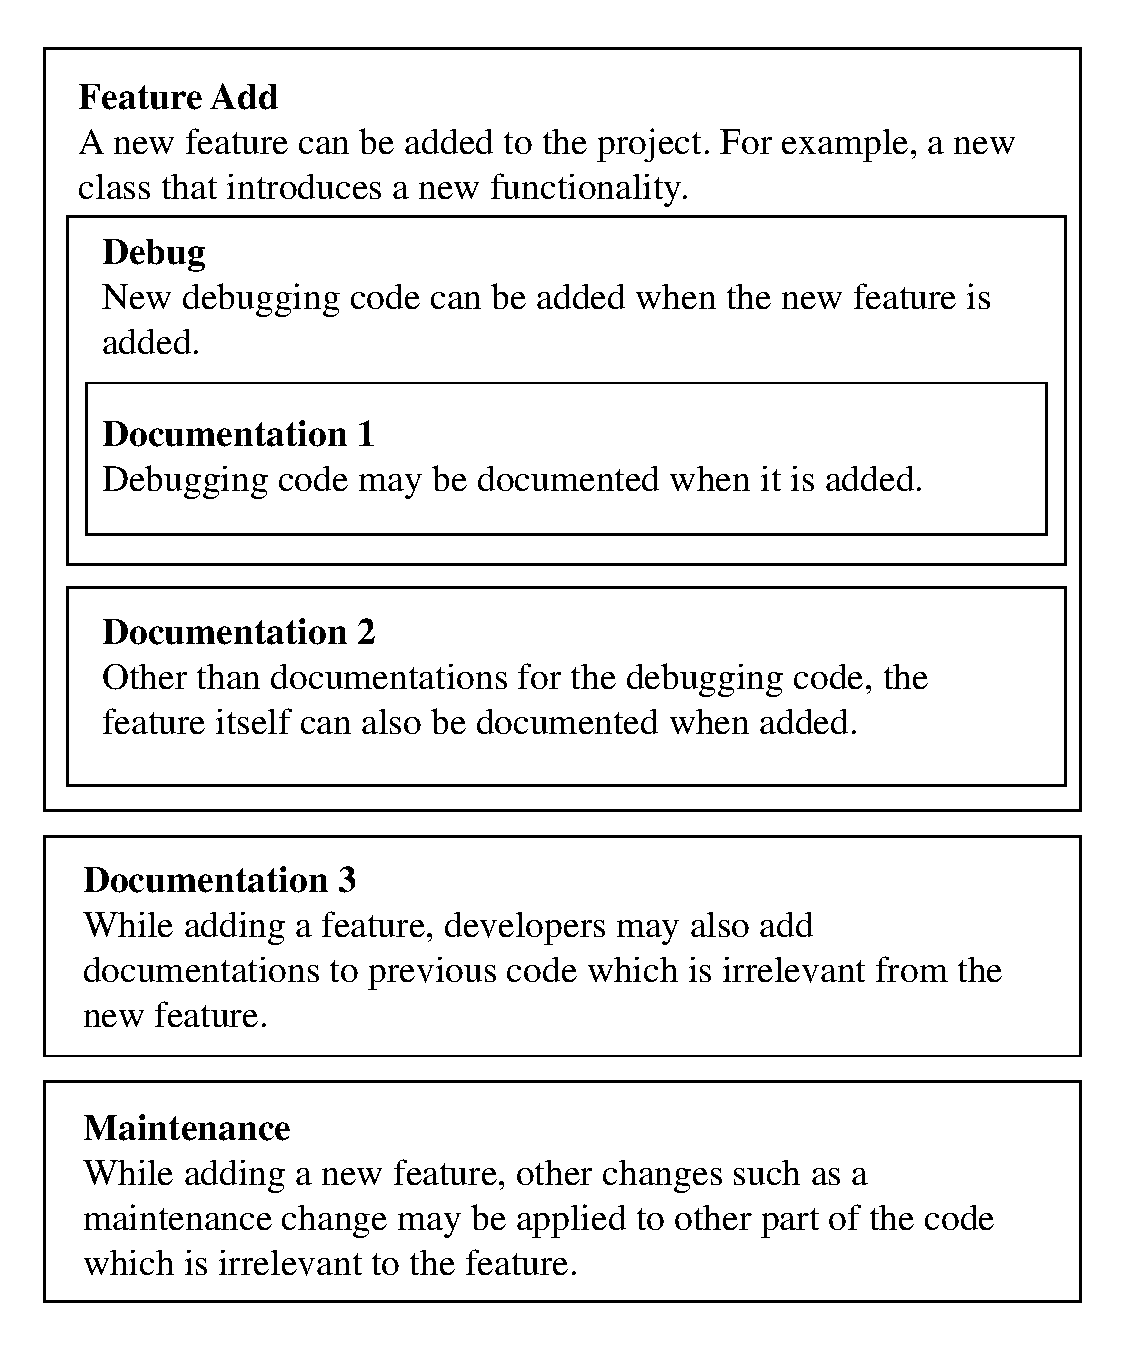
\includegraphics[scale=0.5]{figures/independent_change.pdf}}
\caption{Explanation For Independent Change}
\label{fig:Relationship}
\end{figure}

To improve our tagging, we first note that the original change type definitions overlap. For example, a documentation change may occur as part of a feature add commit. This increases tagging ambiguity and complexity, which we solve by introducing the concept of an \textit{independent change}.

We call a change an \textit{independent change} when it is not a part of other changes.
Fig. \ref{fig:Relationship} explains this concept. It illustrates a commit with multiple changes, in which a new feature contains three sub-changes.
Each block represents a code change. 
In the figure, a new feature change contains debugging code, documentation 1 for the functionality of the feature, documentation 2 for the debugging code, an irrelevant documentation 3, and an irrelevant maintenance change. 
In this case, the debugging code and documentation 1 and 2 are sub-changes to the new feature. 
As a result, we only assign a ``Feature Add'' tag to the new feature instead of assigning tags to all sub-changes. 
As documentation 3 and maintenance are both unrelated to the new feature, they will be assigned Documentation and Maintenance tags.
The new feature, documentation 3, and maintenance groups are independent changes, with the associated three independent tags forming a label the commit. 
With the introduction of independent change types, we reduce the ambiguity in the initial taxonomy which results in fewer cross-validation errors and improved tagging efficiency.





\subsection{Single-tagged Commit And Multi-tagged Commit}

When reviewing manual tagging, we analyze commits with different numbers of tags separately. 
The commits are divided into two groups: \textit{single-tagged} and \textit{multi-tagged}. \textit{Single-tagged} commits contain only one independent change, and \textit{multi-tagged} more than one. 

Fig. \ref{fig: cat_distribution} shows the tag-distributions of single and multi-tagged commits by commit purpose.
In the figure, black bars represent the rates when a certain commit is tagged a single category while gray bars are used to denote multi-tagged. For example, approximately 80\% commits are tagged Testing and more than 95\% of them are multi-tagged commits.
As shown in the figure, Build, Feature Add, Indentation, Refactoring, Testing arise more frequently in multi-tagged commits, indicating these tags tend to appear together with other tags. 
More than 95\% of testing commits have multiple tags, which is consistent with development practices of including the testing code along with most changes.
Documentation is more frequent in single-tagged commits, indicating that many documentation changes are added independently.
As the change of documentation is usually used to explain changed code, this may also imply that contributors often forget to add enough documentation when they accomplish a commit.
For other categories there are no apparent differences between single-tagged and multi-tagged commits.
In addition to comparing these two sets, we also study how many tags each commit has and its distribution. 
\begin{figure*}[htbp]
\centerline{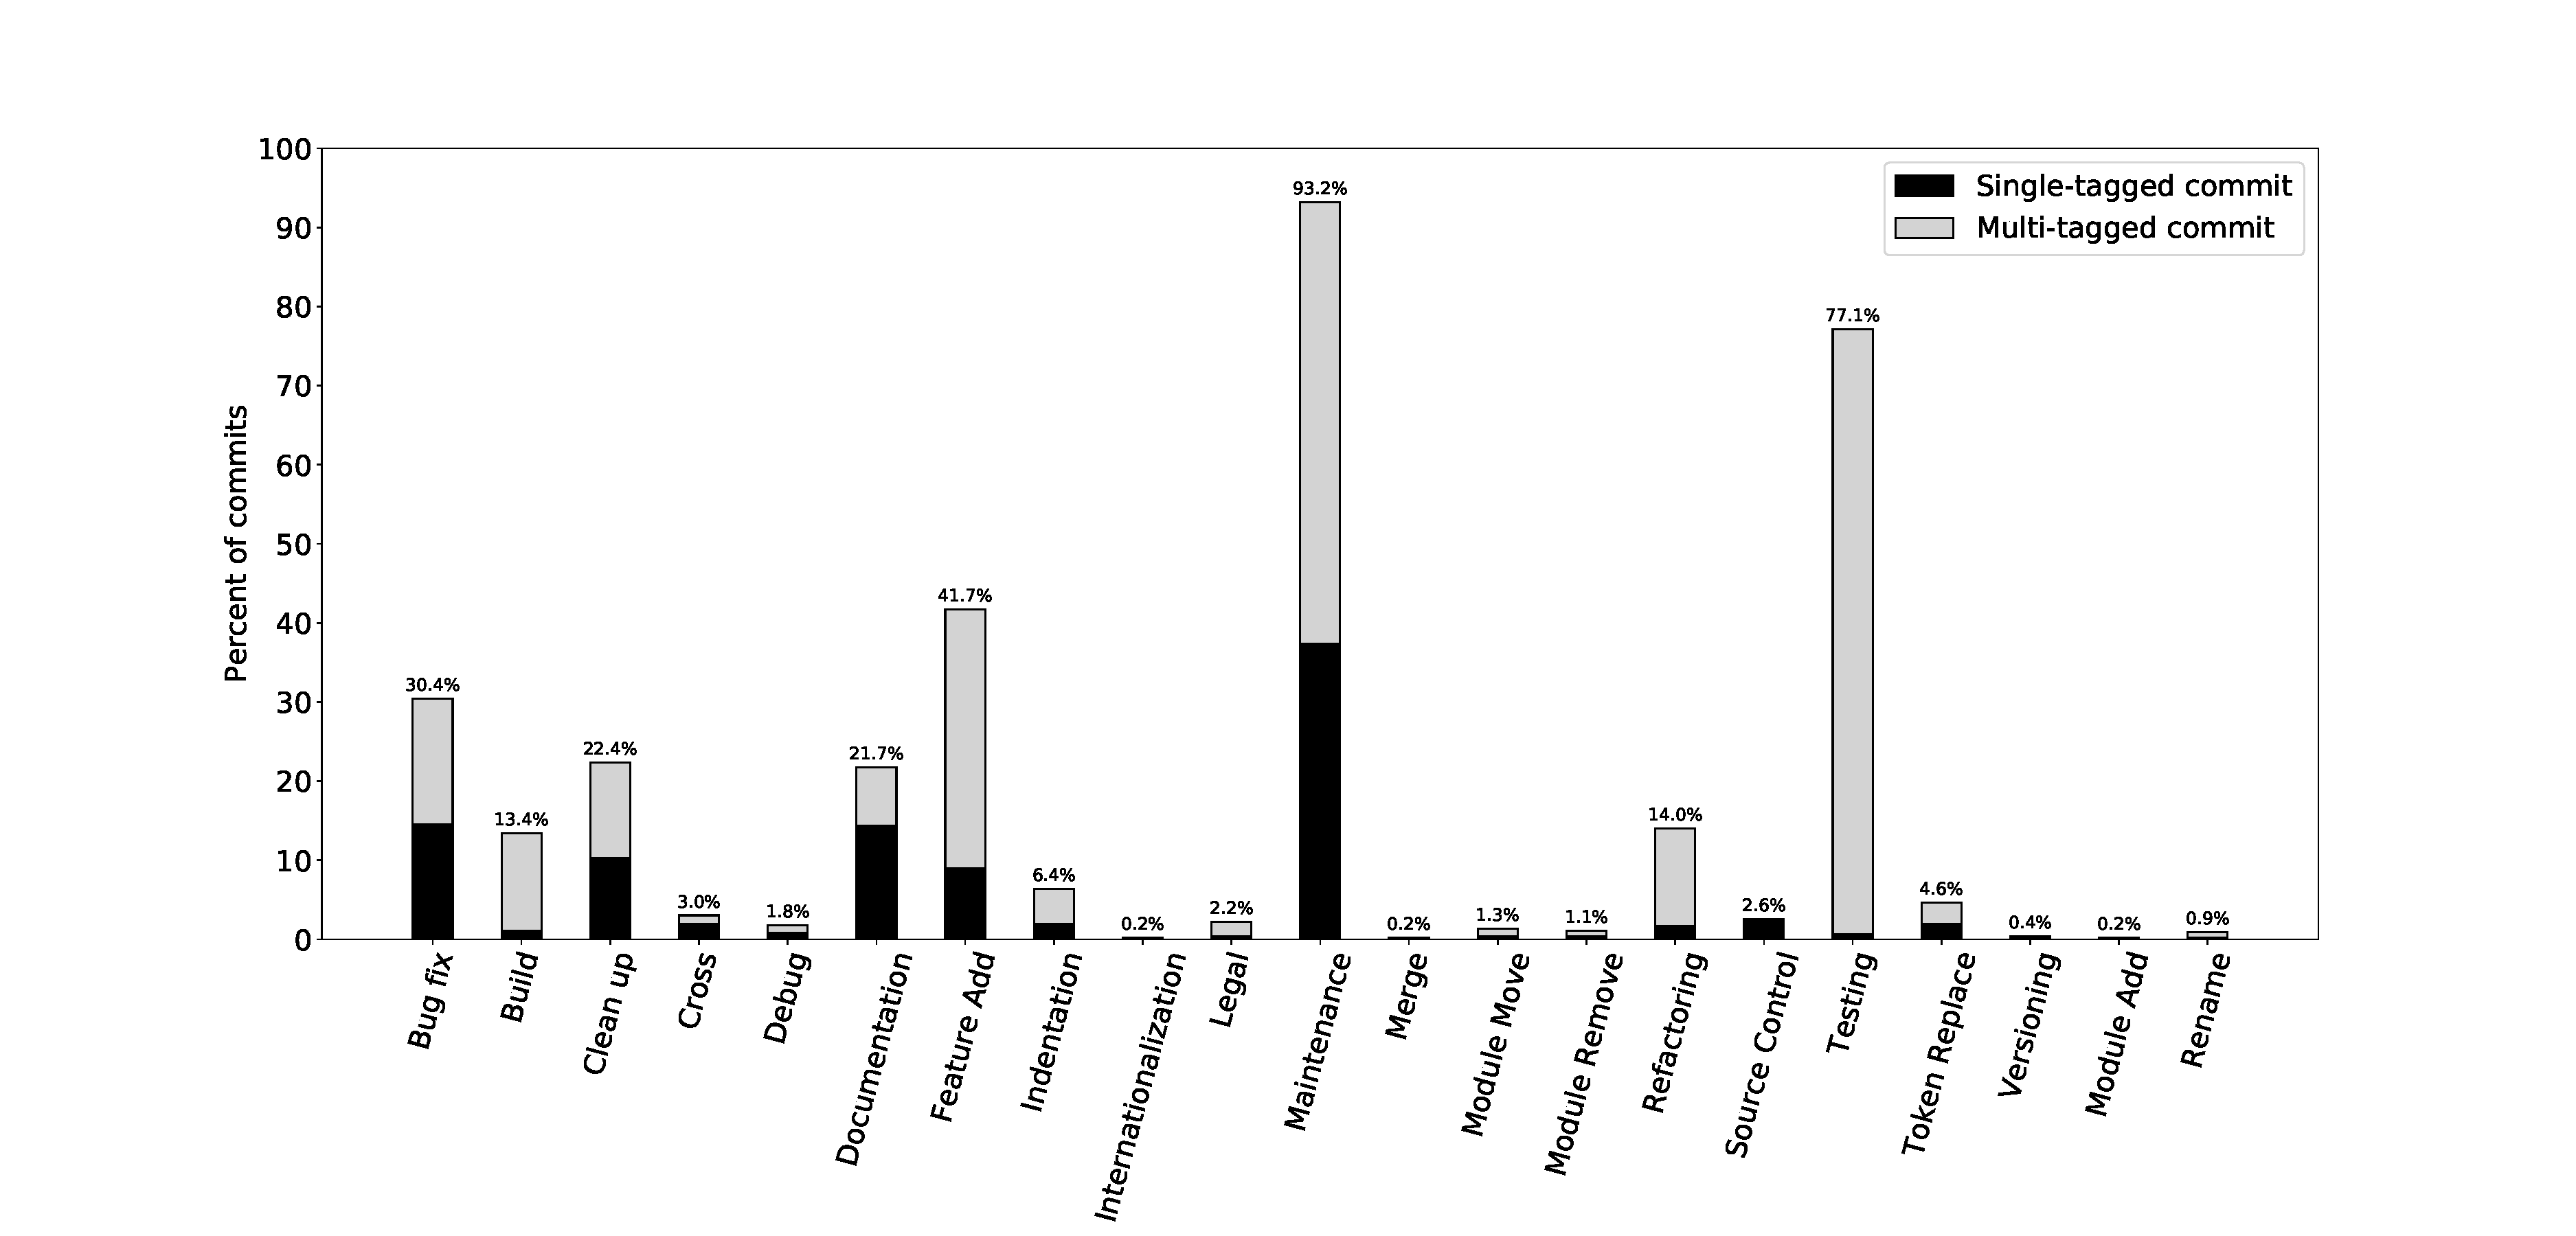
\includegraphics[scale=0.30]{figures/cat_distribution_over_s&m_commits.pdf}}
\caption{Change Type Distribution Between Single-tagged and Multi-tagged Commit}
\label{fig: cat_distribution}
\end{figure*}



\subsubsection{Tag Distribution}
We analyze the differences between the breaker set and the neutral set in terms of tag distributions.
Recall that we call a commit a breaker if it breaks the compilabilty of a compilable revision.
If a commit changes an uncompilable revision and produce another uncompilable revision we do not consider it as a breaker.
We also call a commit a neutral if it changes a compilable revision and produces another compilable revision.
If a commit fixes compile errors of an uncompilable commit we do not consider it as a neutral.

\begin{figure}[htbp]
\centerline{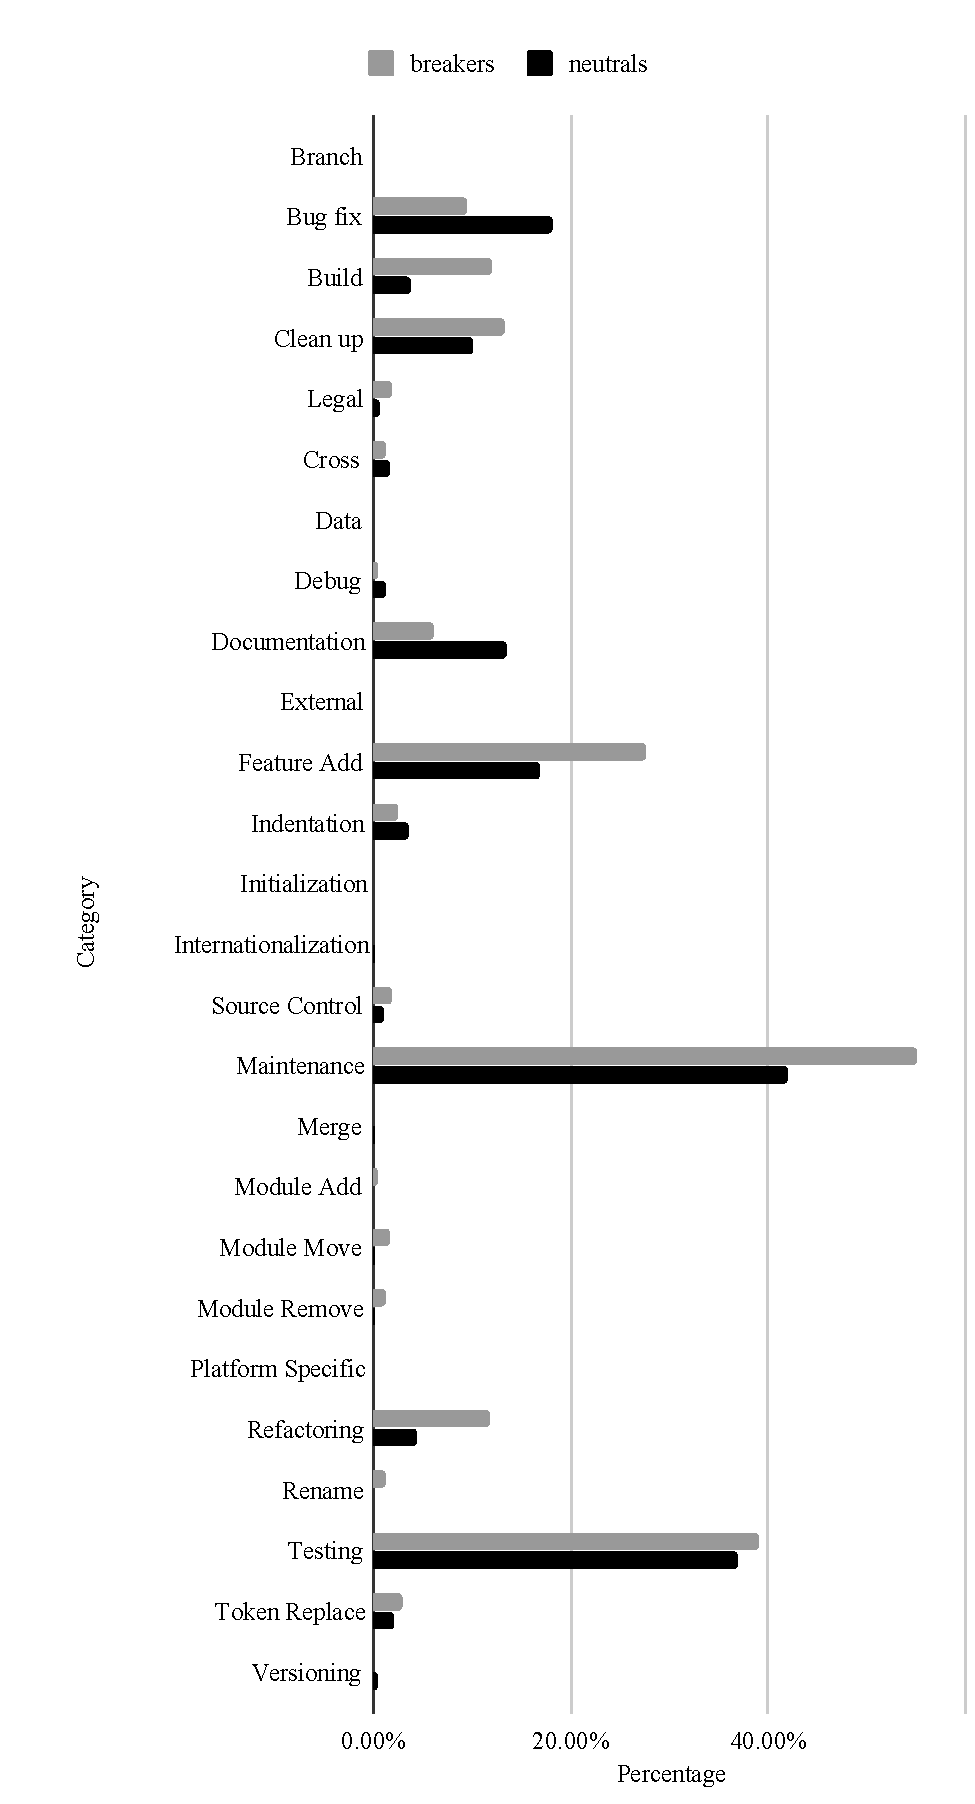
\includegraphics[scale=0.5]{figures/breaker_neutral.pdf}}
\caption{Tag-distribution for Neutrals and Breakers}
\label{fig:breaker_neutral_distribution}
\end{figure}

Fig. \ref{fig:breaker_neutral_distribution} shows the tag-distributions of breaker{}s and neutral{}s with regard to their commit purpose.
Each bar stands for the occurrence rates of that category. 
For example, around 40\% of breaker{}s and neutral{}s are tagged Testing. 
Since a commit could have multiple independent changes, values for one color may add up to more than 100\%.
The presence ratios for Bug Fix, Documentation, is higher in the neutrals while Feature Add, Build, Refactoring, Clean up and Maintenance is higher in breaker{}s.
The breaker{}s have 1.90 tags on average while neutral{}s have 1.56 on average.


\begin{table}[htbp]
    \centering
    \caption{Ratio of Compilable Commits Over Neutrals and Breakers}
      \begin{tabular}{llll}
      \hline
      \multirow{2}[4]{*}{\textbf{Category}} & \multicolumn{3}{l}{\textbf{Compilablity}} \\          & \textbf{Neutral(\%)} & \textbf{Breaker(\%)} & \textbf{p-value} \\
      \hline
      \textbf{Branch} & 0.00  & 0.00  & - \\
      \hline
      \textbf{Bug fix} & 18.17  & 9.55  & \textbf{0.000} \\
      \hline
      \textbf{Build} & 3.67  & 12.10  & \textbf{0.000} \\
      \hline
      \textbf{Clean up} & 10.00  & 13.38  & 0.150  \\
      \hline
      \textbf{Cross} & 1.67  & 1.27  & 0.781  \\
      \hline
      \textbf{Data} & 0.00  & 0.00  & - \\
      \hline
      \textbf{Debug} & 1.17  & 0.32  & 0.276  \\
      \hline
      \textbf{Documentation} & 13.50  & 6.05  & \textbf{0.005} \\
      \hline
      \textbf{External} & 0.00  & 0.00  & - \\
      \hline
      \textbf{Feature Add} & 16.83  & 27.71  & \textbf{0.000} \\
      \hline
      \textbf{Indentation} & 3.50  & 2.55  & 0.552  \\
      \hline
      \textbf{Initialization} & 0.00  & 0.00  & - \\
      \hline
      \textbf{Internalization} & 0.17  & 0.00  & 1.000  \\
      \hline
      \textbf{Legal} & 0.67  & 1.91  & 0.101  \\
      \hline
      \textbf{Maintenance} & 41.83  & 55.10  & \textbf{0.000} \\
      \hline
      \textbf{Merge} & 0.17  & 0.00  & 1.000  \\
      \hline
      \textbf{Module Add} & 0.00  & 0.32  & 0.344  \\
      \hline
      \textbf{Module Move} & 0.17  & 1.59  & \textbf{0.020} \\
      \hline
      \textbf{Module Remove} & 0.17  & 1.27  & \textbf{0.050} \\
      \hline
      \textbf{Platform Specific} & 0.00  & 0.00  & - \\
      \hline
      \textbf{Refactoring} & 4.33  & 11.78  & \textbf{0.000} \\
      \hline
      \textbf{Rename} & 0.00  & 1.27  & \textbf{0.014} \\
      \hline
      \textbf{Source Control} & 1.00  & 1.91  & 0.358  \\
      \hline
      \textbf{Testing} & 36.83  & 39.17  & 0.518  \\
      \hline
      \textbf{Token Replace} & 2.00  & 2.87  & 0.486  \\
      \hline
      \textbf{Versioning} & 0.33  & 0.00  & 0.549  \\
      \hline
      \end{tabular}%
    \label{tab:breaker_neutral}%
  \end{table}%

Again, we perform odd ratio test (the Fisher's Exact Test) to study the correlation between categories and compilability. 
According to the test result shown in Table \ref{tab:breaker_neutral}, we found that Bug Fix, Build, Documentation, Feature Add, Maintenance, Module Move, Module Remove, Refactoring, Rename have significant differences between breaker{}s and neutral{}s, which is consistent with the results of Fig.\ref{fig:breaker_neutral_distribution}.



\subsection{Single-tagged Commit And Multi-tagged Commits}

Recall that we call a commit with multiple independent changes \textit{multi-tagged} and a commit with only one independent change \textit{single-tagged}.

Almost 50\% of our analyzed commits are multi-tagged.
We summarize the number of tags for each commit independently for the breaker and the neutral set, as shown in Fig. \ref{fig:num_tasks_fig}. 
The figure shows the distributions of commits with different numbers of tags in the breaker{}s or neutral{}s. 
Each bar stands for the ratio of presence of commits with certain number of tags.

For example, 55\% of neutral{}s only have one tag. 
The curves are Kernel Density Estimations of these two distributions that are long tail distributions. 
The number of instances decreases as the number of tags increases.
As for its relation with compilability, we can see a neutral is more likely to have a small number of tags while a breaker has a relatively large one. 
We also use the Kernel Density Estimation (KDE) to estimate these two distributions. 
The distribution density curve of neutral{}s is sharper than breaker{}s which means the proportion of commits decreases more sharply in the neutral{}s than in the breaker{}s with increase of the number of tags. 
We can interpret it as a commit is more likely to break its compilability when it has more tags.

\begin{figure*}[htbp]
\centerline{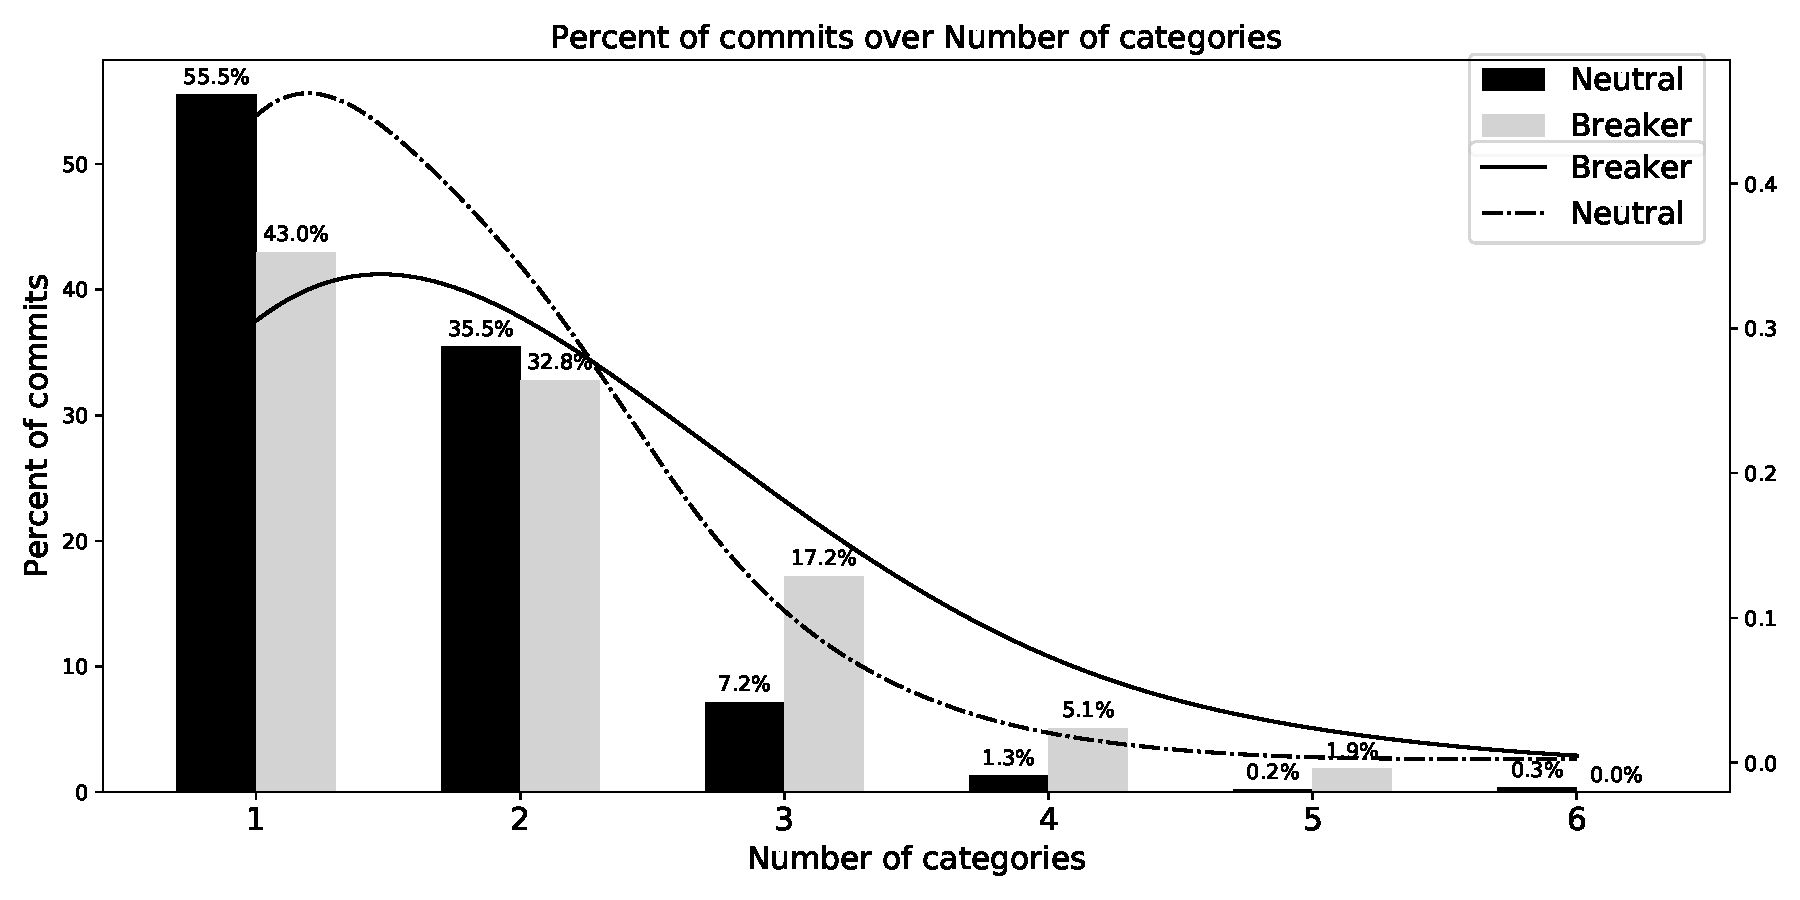
\includegraphics[scale=0.6]{figures/num_tasks_break_rate.pdf}}
\caption{Compilability With Number of Tags in Each Commit}
\label{fig:num_tasks_fig}
\end{figure*}



\subsubsection{Small And Large Commits}

We also analyze the relation between uncompilability and whether a commit is large or small. 
We draw boxplot of changed Lines of Code (LOC) for breaker set and neutral set which is shown in Fig. \ref{fig: commit_LOC}.
Fig. \ref{fig: commit_LOC}(a) shows the distributions of neutrals and breakers respectively. 
(b) shows distributions of commits with different number of tags respectively. 
In boxplot, each box represents inter-quartile range (IQR) of data points, the range of major part of data and circle represents outlier of data points which are outside 1.5 IQR.
As shown in Fig. \ref{fig: commit_LOC}(a), the distribution of breaker{}s is shifted upward from the distribution of neutral{}s and it means breaker{}s tend to have larger changed LOC than neutral{}s. 
This indicates larger commits are more likely to result in compilation breach.

We also analyze the distribution of changed LOC for commits which contains different number of tags as shown in Fig. \ref{fig: commit_LOC}(b).
The result shows that if a commit contains more tags, it tends to have more lines of code changed. 
\begin{figure*}[htbp]
\centerline{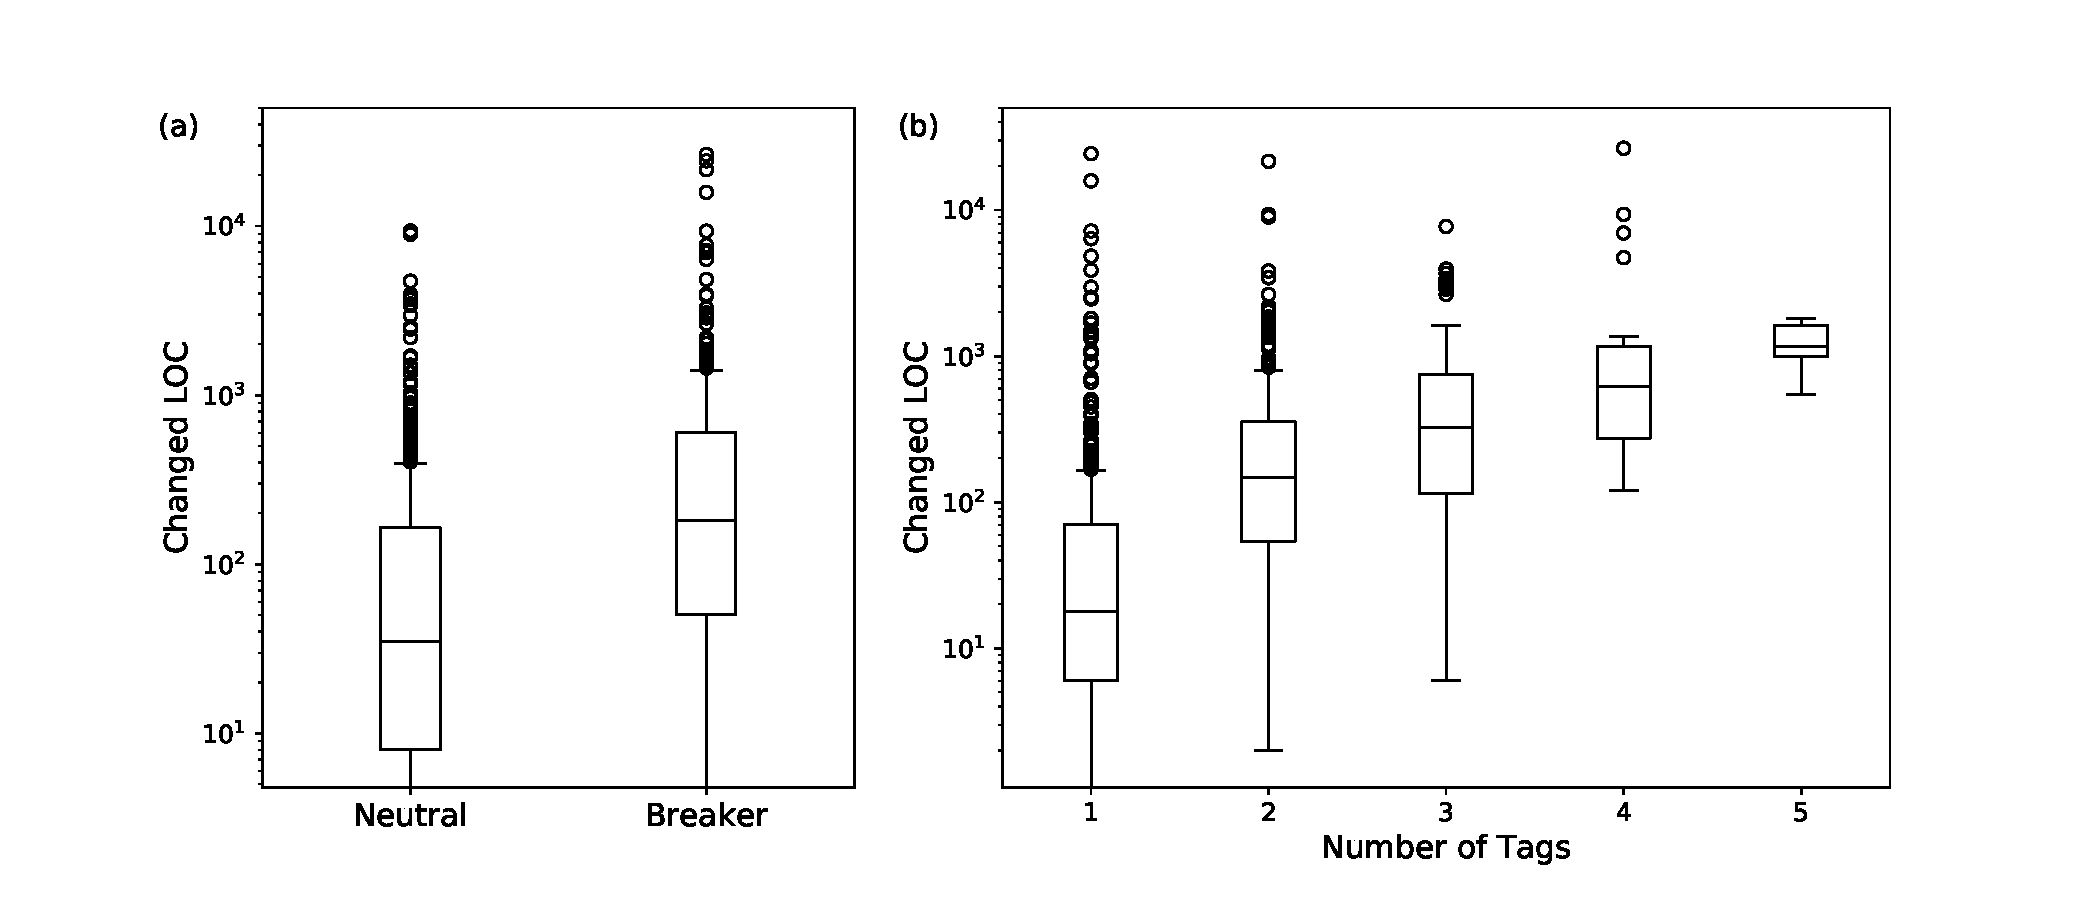
\includegraphics[scale=0.5]{figures/commit_size.pdf}}
\caption{Commits Distribution Over Lines of Code.}
\label{fig: commit_LOC}
\end{figure*}
